\section{Exercise 1}
\textit{Try setting your own scene with camera, light source(s), and back-ground. And put (an) object(s) in the scene! Adjust your settings till you are satisfied with the scene! For now, if you don’t add in any object modifiers, your object would just look like a solid black block. But that’s okay! In what follows, we will introduce some object modifiers,which will add surface properties and textures to your object(s).}
See \autoref{fig:ex1}.

\begin{figure}[h]
  \centering
  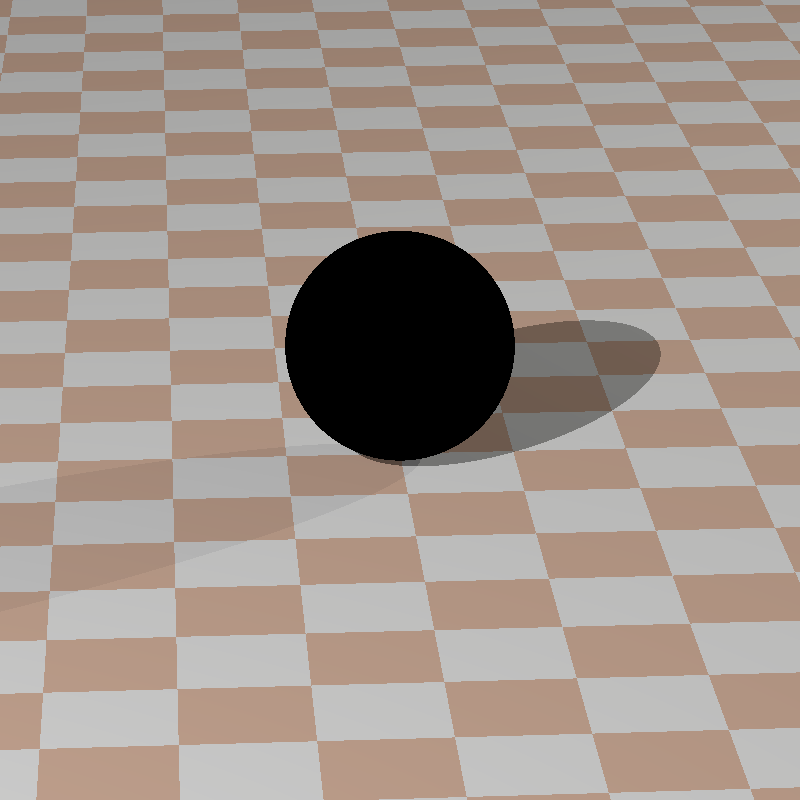
\includegraphics[height=5cm]{ex1.png}
  \caption{Solution for Exercise 1}
  \label{fig:ex1}
\end{figure}